%%%%%%%%%%%%%%%%%%%%%%% file template.tex %%%%%%%%%%%%%%%%%%%%%%%%%
%
% This is a general template file for the LaTeX package SVJour3
% for Springer journals.          Springer Heidelberg 2010/09/16
%
% Copy it to a new file with a new name and use it as the basis
% for your article. Delete % signs as needed.
%
% This template includes a few options for different layouts and
% content for various journals. Please consult a previous issue of
% your journal as needed.
%
%%%%%%%%%%%%%%%%%%%%%%%%%%%%%%%%%%%%%%%%%%%%%%%%%%%%%%%%%%%%%%%%%%%
%
% First comes an example EPS file -- just ignore it and
% proceed on the \documentclass line
% your LaTeX will extract the file if required
% \begin{filecontents*}{example.eps}
% %!PS-Adobe-3.0 EPSF-3.0
% %%BoundingBox: 19 19 221 221
% %%CreationDate: Mon Sep 29 1997
% %%Creator: programmed by hand (JK)
% %%EndComments
% gsave
% newpath
%   20 20 moveto
%   20 220 lineto
%   220 220 lineto
%   220 20 lineto
% closepath
% 2 setlinewidth
% gsave
%   .4 setgray fill
% grestore
% stroke
% grestore
% \end{filecontents*}
%
\RequirePackage{fix-cm}

\documentclass[smallextended]{svjour3}

\smartqed  % flush right qed marks, e.g. at end of proof
%

\usepackage{tabularx}

\usepackage{graphicx}

\usepackage[authoryear]{natbib}  %% The order is important

\usepackage[resetlabels]{multibib}
\newcites{inappendix}{Supplementary References}

% \usepackage{alifeconf}

\usepackage{hyperref}

\usepackage{subcaption}

\usepackage{hhline}

\usepackage{amsmath}

\usepackage{rotating}

\usepackage{bibspacing}
\setlength{\bibsep}{0pt plus 0.3ex}

\ifdefined\mydraft
\mydraft
\fi

% \usepackage[
%   %subtle
%   moderate
% ]{savetrees}

\graphicspath{{img/}}

% *****************
%  Requirements:
% *****************
%
% - All pages sized consistently at 8.5 x 11 inches (US letter size).
% - PDF length <= 8 pages for full papers, <=2 pages for extended
%    abstracts.
% - Abstract length <= 250 words.
% - No visible crop marks.
% - Images at no greater than 300 dpi, scaled at 100%.
% - Embedded open type fonts only.
% - All layers flattened.
% - No attachments.
% - All desired links active in the files.

% Note that the PDF file must not exceed 5 MB if it is to be indexed
% by Google Scholar. Additional information about Google Scholar
% can be found here:
% http://www.google.com/intl/en/scholar/inclusion.html.


% If your system does not generate letter format documents by default,
% you can use the following workflow:
% latex example
% bibtex example
% latex example ; latex example
% dvips -o example.ps -t letterSize example.dvi
% ps2pdf example.ps example.pdf


% For pdflatex users:
% The alifeconf style file loads the "graphicx" package, and
% this may lead some users of pdflatex to experience problems.
% These can be fixed by editing the alifeconf.sty file to specify:
% \usepackage[pdftex]{graphicx}
%   instead of
% \usepackage{graphicx}.
% The PDF output generated by pdflatex should match the required
% specifications and obviously the dvips and ps2pdf steps become
% unnecessary.


% Note:  Some laser printers have a serious problem printing TeX
% output. The use of ps type I fonts should avoid this problem.


\title{Matchmaker, Matchmaker, Make Me a Match: Geometric, Variational, and Evolutionary Implications of Criteria for Tag Affinity}
\titlerunning{Matchmaker, Matchmaker, Make Me a Match}
\author{
    Matthew Andres Moreno
	  \and Alexander Lalejini
    \and Charles Ofria \\
}

\authorrunning{Moreno et al.} % if too long for running head

\institute{%
  M. A. Moreno \at
  BEACON Center for the Study of Evolution in Action \\
  Department of Computer Science and Engineering \\
  Program in Ecology, Evolutionary Biology, and Behavior \\
  Michigan State University, East Lansing, MI \\
  \email{mmore500@msu.edu}
\and
  A. Lalejini \at
  University of Michigan, Ann Arbor, MI
\and
  C. Ofria \at
  BEACON Center for the Study of Evolution in Action \\
  Department of Computer Science and Engineering \\
  Program in Ecology, Evolutionary Biology, and Behavior \\
  Michigan State University, East Lansing, MI \\
}

\date{Received: date / Accepted: date}

% For several authors from the same institution use the same number to
% refer to one address.
%
% If the names do not fit well on one line use
%         Author 1, Author 2 ... \\ {\Large\bf Author n} ...\\ ...
%
% If the title and author information do not fit in the area
% allocated, place \setlength\titlebox{<new height>} after the
% \documentclass line where <new height> is 2.25in

% pragma once, adapted from https://tex.stackexchange.com/a/195173
\makeatletter
\let\pragma@iinput=\@iinput
\def\@iinput#1{\xdef\@pragmafile{#1}\pragma@iinput{#1}}
\def\@pragmafile{default}
\def\pragmaonce{%
   \csname pragma@\@pragmafile\endcsname
   \global\expandafter\let \csname pragma@\@pragmafile\endcsname = \endinput
}
\makeatother

\begin{document}
\maketitle

\begin{abstract}

Genetic programming and artificial life systems commonly employ tag-matching schemes to determine interactions between model components.
%Criteria to determine affinity between tags %TODO
However, the implications of criteria used to determine affinity between tags with respect to constraints on emergent connectivity, canalization of changes to connectivity under mutation, and evolutionary dynamics have not been considered.
We highlight differences between tag-matching criteria with respect to geometric constraint and variation generated under mutation. 
We find that tag-matching criteria can influence the rate of adaptive evolution and the quality of evolved solutions.
Better understanding of the geometric, variational, and evolutionary properties of tag-matching criteria will facilitate more effective incorporation of tag matching into genetic programming and artificial life systems.
By showing that tag-matching criteria influence connectivity patterns and evolutionary dynamics, our findings also raise fundamental questions about the properties of tag-matching systems in nature.

\keywords{Genetic Programming \and Event-driven Genetic Programming \and Tag-based Referencing \and Module-based Genetic Programming \and Artificial Gene Regulatory Networks}
% \PACS{PACS code1 \and PACS code2 \and more}
% \subclass{MSC code1 \and MSC code2 \and more}

\end{abstract}


\section{Introduction} \label{sec:introduction}

Genetic programming often requires operations to undergo evolutionary adjustment of which operands they act upon.
This process can tweak the semantics of existing evolved code, critical in particular for duplication and divergence processes commonly highlighted in discussions of evolvability \citep{altenberg1994evolution}.
This process also allows for incorporation and removal of operands.
Additionally, dynamic reorganization of code modules can facilitate hierarchical problem-solving \citep{Kinnear:Koza:1994:adf}.

Tag-based referencing, also known as ``pattern matching'' or ``inexact referencing,'' offers a practical solution for choosing computational operands.
This approach attaches a tag to each computational operand and query.
Operands are then selected for each query according to compatibility between respective tags.
For example, consider a system where matching is performed according to absolute difference between integer tags.
If two operands tagged 8 and 2 are available, a query tagged 7 would retrieve the operand tagged 8.
Conversely, a query tagged 2 would retrieve the operand tagged 2.

Inexact referencing techniques are widely used in agent-based modeling \citep{riolo2001evolution}, neuroevolution \citep{reisinger2007acquiring}, artificial gene regulatory networks \citep{banzhaf2003artificial}, and genetic programming \citep{spector2011tag, lalejini2018evolving}.
Some existing work attempts to distinguish tag-matching criteria through narrative explanations of evolutionary properties and biological analogies \citep{downing2015intelligence,scherer2004activation}, our work provides the first systematic, quantitative, and empirical insight into the consequences of commonly used tag-matching criteria.

\section{Methods}

Rigorous comparison of disparate tag-matching schemes required careful standardization of tag representation, mutation, and match scoring.
We used 32-bit bitstrings as tags for all experiments.
Mutations toggled individual bits stochastically at a uniform per-bit rate.
Match distances were normalized to ensure a uniform distribution of scores between randomly sampled tags.
This ensured consistent and intuitive interpretation across all tag-matching metrics.

\begin{table*}[!htbp]
\begin{tabularx}{\textwidth}{l|X}
\textbf{Metric}       & \textbf{Description}                                                                                                                                        \\ \hline
Hash                  & SHA1 cryptographic hash of  concatenation of \texttt{tag\_0} and \texttt{tag\_1} \citep{eastlake2001us}                         \\ \hline
Hamming               & fraction of positions within \texttt{tag\_0} and \texttt{tag\_1} with mismatching bits                                                                         \\ \hline
Integer               & value added to the unsigned integer representation of \texttt{tag\_0} to reach representation of \texttt{tag\_1}, wrapping around if necessary \\ \hline
Bidirectional Integer & lesser of integer metric distances \texttt{d(tag\_0, tag\_1)} and \texttt{d(tag\_1, tag\_0)}                                                                \\ \hline
Streak                & ratio of lengths of contiguously matching and mismatching substrings \\ \hline
\end{tabularx}

% \begin{tabularx}{\textwidth}{l|X|X}
% \hline
% \textbf{Metric}       & \textbf{Commutative?} & \textbf{Multidimensional?} \\ \hline
% Hash                  & no                    & yes                        \\ \hline
% Hamming               & yes                   & yes                        \\ \hline
% Streak                & yes                   & yes                        \\ \hline
% Integer               & no                    & no                         \\ \hline
% Bidirectional Integer & yes                   & no
% \end{tabularx}

\caption{
Surveyed tag-matching metrics.
}
\label{tab:metrics}
\vspace{-6ex}
\end{table*}


We compared five tag-matching metrics: Hamming, hash, integer, bidirectional integer, and streak (Table \ref{tab:metrics}).
We included the Hamming and bidirectional integer metrics because of their ubiquity in genetic programming.
We included the integer metric due to its use in prior tag-matching studies \citep{spector2011tag,spector2012tag}.
The streak metric has been proposed to model large-effect mutations observed in biology \cite{downing2015intelligence}.
We introduce the hash metric as a control that has no geometric structure, in contrast to all other metrics.

All tag-matching algorithms appear in the Empirical C++ library \citep{charles_ofria_2019_2575607} as interchangeable components of the MatchBin tool suite.

\section{Summary of Results}

% We explored how these tag-matching schemes differ with respect to
% (1) \textit{geometric structure} that biases or limits the patterns of connectivity that form among queries and operands, (2) \textit{variational properties} that influence changes to connectivity observed under mutation, and (3) \textit{evolutionary outcomes} such as the rate of adaptive evolution and the quality of evolved solutions.

\subsection{Geometric and Variational Analyses}

We first investigated the impact of different tag-matching metrics on mutational neighborhoods and geometric constraints of connectivity patterns.
Single-step and multi-step mutational analyses allowed us to characterize the local and broader mutational landscapes induced by each metric.
The integer metrics displayed the most restrictive geometric structure, followed by the Hamming and streak metrics.
Such restrictive structure limits possible connectivity patterns between tagged components, for instance precluding a pair of query tags that both closely match one operand tag from strongly disagreeing in match affinity to other operand tags.

Single-step mutational analyses showed large-effect one-step mutations under the hash, integer, and streak metrics, but not under the Hamming metric.
For multi-step mutational analyses, match affinity decayed most rapidly along mutational walks under the integer metrics and the control hash metric.
Match affinity decayed slowest along mutational walks under the Hamming metric, while the streak metric degraded second-slowest.

Interestingly, our results contradict existing hypotheses of the streak metric's mutational properties, which propose greater robustness compared to the Hamming metric \citep{downing2015intelligence}.
This discrepancy arises from our normalization to ensure a uniform distribution of raw match scores.
We believe our result to be more representative, as normalized match distance corresponds to the probability that arbitrary tags would match more strongly by chance.
This directly relates to how effectively an operand tag competes to be the ``best'' match for a query.

\subsection{Evolutionary Experiments}

Next, we investigated the performance of various tag-matching metrics in digital evolution, starting with a toy problem and progressing to the more complex, applied domain of the SignalGP genetic programming representation.
In the toy problem, we define a target connection topology between tagged queries and operands.
We instantiate a population of tag sets and select for those with tag-match pairs that correspond to target topology components.
Across experiments, we systematically varied the target topological density, comparing scenarios with low constraint (i.e., each query selected to match with a single operand) and high constraint (i.e., each query selected to match with multiple operands).

In the SignalGP problem domain, tag-based referencing facilitates activation of modules (functions) in response to exogenously- and endogenously-generated signals.
Tags specify the relationship between signals and signal-handlers (program modules), triggering the module with the closest matching tag to run its linear sequence of instructions.
The instruction set includes traditional GP operations, instructions to generate arbitrarily-tagged internal and external signals, as well as module promoter and repressor instructions to facilitate during-lifetime plasticity as described in \cite{lalejini2021tag}.

We perform experiments with two diagnostic SignalGP problems: the changing-signal task which selects for sparse tag interactions (low constraint) and the directional-signal Task which selects for denser tag interactions (high constraint).

The Hamming and streak metrics performed best in the SignalGP experiments.
In the high-constraint directional-signal task, the streak metric outperformed the Hamming metric.
The hash metric showed the next-best performance, yielding more solutions than the integer metrics, which both performed comparably poorly.

Interestingly, the hash metric performed best in low-constraint target-matching experiments, likely due to its strong variation-generation capacity.
However, the hash metric was outperformed in low-constraint SignalGP experiments by the streak and Hamming metrics.
Similarly, the integer metrics were outperformed by the streak and Hamming metrics in low-constraint SignalGP experiments, despite their good performance in low-constraint target-matching experiments.

It remains unclear what aspect of the genetic programming experiments selectively stymy the hash and integer metrics.
Possibilities include better streak and Hash support for duplication and differentiation processes along SignalGP lineages or differences in fitness landscape ruggedness.
Further experiments are needed to understand the evolutionary dynamics of non-trivial tag-matching systems and the interplay of those dynamics with tag-matching metrics.

\section{Conclusion}

In a first step toward systematic theory for evolutionary applications of tag-matching, we have cataloged mechanistic differences between tag-matching criteria and demonstrated significant impact of these differences on adaptive evolution.
This work provides practical guidance on tag-matching metrics and mutation rates that can be applied to existing genetic programming systems.
Important open questions remain, such as the relationships between tag-matching criteria and specificity, modularity, robustness, and the process of duplication and divergence.
Evolvability or information-theoretical analyses may prove fruitful in exploring these questions.
A framework for the systematic design of new tag-matching metrics and mutation operators with desirable evolutionary properties should also be pursued.

Tag-like mechanisms mediate interaction and function across various biological scales.
Investigating the mechanistic and evolutionary properties of tagging systems promises more nuanced understanding and algorithmic emulation of natural systems.


% \section{Software and Data Availability}

We implemented our experimental systems using the Empirical library for scientific software development in C++, available at \url{https://github.com/devosoft/Empirical} \citep{charles_ofria_2019_2575607}.
The code used to perform and analyze our experiments, our figures, and data from our experiments is available via the Open Science Framework at \url{https://osf.io/gw5mc/} \citep{foster2017open}.


\section*{Funding}

This research was supported in part by NSF grants DEB-1655715 and DBI-0939454.
This material is based upon work supported by the National Science Foundation Graduate Research Fellowship under Grant No. DGE-1424871.


\section*{Conflict of interest}

The authors declare that they have no conflict of interest.

\section*{Availability of data and material}

The code used to perform and analyze our experiments, our figures, and data from our experiments is available via the Open Science Framework at \url{https://osf.io/gw5mc/} \citep{foster2017open}.
Data and figures are also organized alongside related manuscript source files at \url{https://github.com/mmore500/tag-olympics-writeup}. 

\section*{Code availability} 

We implemented our experimental systems using the Empirical library for scientific software development in C++, available at \url{https://github.com/devosoft/Empirical} \citep{charles_ofria_2019_2575607}.
Software written for these experiments is available at \url{https://github.com/amlalejini/Exploring-tag-matching-metrics-in-SignalGP/tree/1.0} and \url{https://github.com/mmore500/tag-olympics}.

\section*{Authors' contributions} Matthew Andres Moreno and Alexander Lalejini contributed to the study conception and design.
Material preparation, data collection and analysis of genetic programming benchmarks were performed by Alexander Lalejini.
Other material preparation, data collection and analysis of genetic programming benchmarks were performed by Matthew Andres Moreno.
The first draft of the manuscript was written by Matthew Andres Moreno and Alexander Lalejini and all authors commented on previous versions of the manuscript.
All authors read and approved the final manuscript.


\section{Acknowledgements}

Thanks to members of the DEVOLAB, in particular TODO for help with TODO.
This research was supported in part by NSF grants DEB-1655715 and DBI-0939454, and by Michigan State University through the computational resources provided by the Institute for Cyber-Enabled Research.
This material is based upon work supported by the National Science Foundation Graduate Research Fellowship under Grant No. DGE-1424871.
Any opinions, findings, and conclusions or recommendations expressed in this material are those of the author(s) and do not necessarily reflect the views of the National Science Foundation.


\footnotesize
\bibliographystyle{apalike}
\bibliography{bibl} % replace by the name of your .bib file

\clearpage
\newpage

\appendix

\setcounter{secnumdepth}{2}


\begin{figure}
\begin{center}

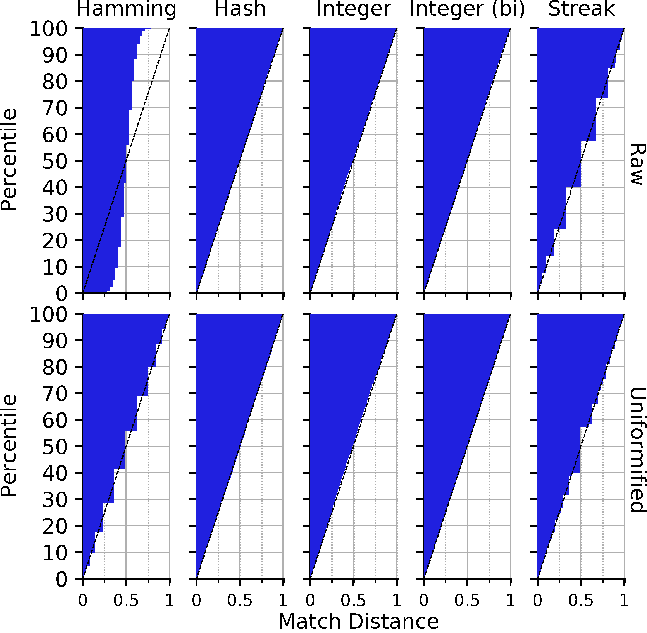
\includegraphics[width=\columnwidth]{img/uniformification/bitweight=0dot5+seed=1+title=low-score-distribution+_data_hathash_hash=75684cf1e73fb7f1+_script_fullcat_hash=c3113c80efb02374+ext=}
\caption{
Distance distributions of metrics before and after uniformification.
Each visualization arranges individually sampled observations (thin horizontal bars) vertically in descending order.
The $y$ axis can be interpreted as ranging form the \nth{0} percentile of outcomes (bottom) to \nth{100} percentile (top) with width of horizontal bars showing match distance at a certain percentile.
Dashed lines trace an ideal uniform distribution.
}
\label{fig:uniformification_supp}

\end{center}
\end{figure}


\begin{figure*}[!htbp]
\begin{center}

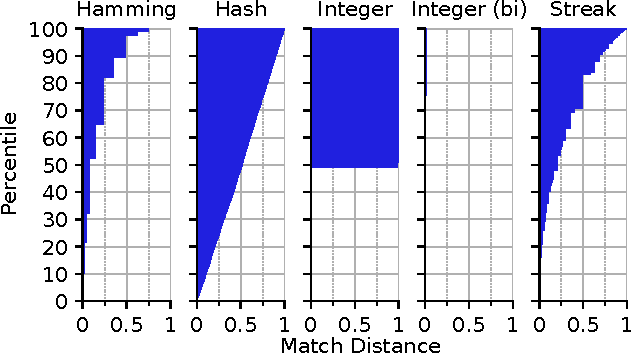
\includegraphics[width=\linewidth]{img/sphere/bitweight=0dot5+seed=1+title=dimensionality_distnplot+_data_hathash_hash=c0f6c5cf854ff253+_script_fullcat_hash=bea2a31376bf6bd0+ext=}
\caption{
Cumulative distributions of sampled similarity constraint values.
Each visualization arranges individually sampled observations (thin horizontal bars) vertically in descending order.
The $y$ axis can be interpreted as ranging from the \nth{0} percentile of outcomes (bottom) to \nth{100} percentile (top) with horizontal bar width showing similarity constraint at a certain percentile.
}
\label{fig:sphere_supp}

\end{center}
\end{figure*}


\begin{figure*}
\begin{center}

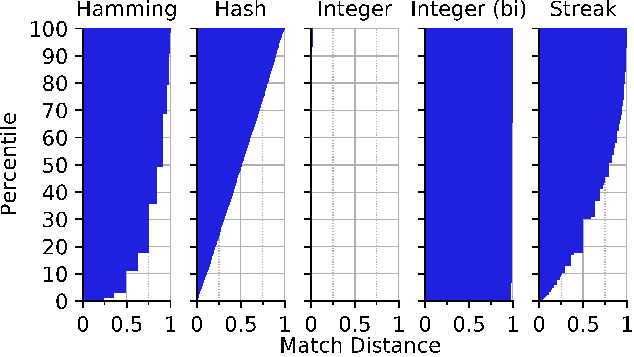
\includegraphics[width=\linewidth]{img/sphere_reverse/bitweight=0dot5+seed=1+title=dimensionality_distnplot+_data_hathash_hash=93f97a11cb443d35+_script_fullcat_hash=bea2a31376bf6bd0+ext=}
\caption{
Cumulative distributions of sampled dissimilarity constraint values.
Each visualization arranges individually sampled observations (thin horizontal bars) vertically in descending order.
The $y$ axis can be interpreted as ranging from the \nth{0} percentile of outcomes (bottom) to \nth{100} percentile (top) with horizontal bar width showing similarity constraint at a certain percentile.
}
\label{fig:sphere_reverse_supp}

\end{center}
\end{figure*}


\begin{figure}
\begin{center}
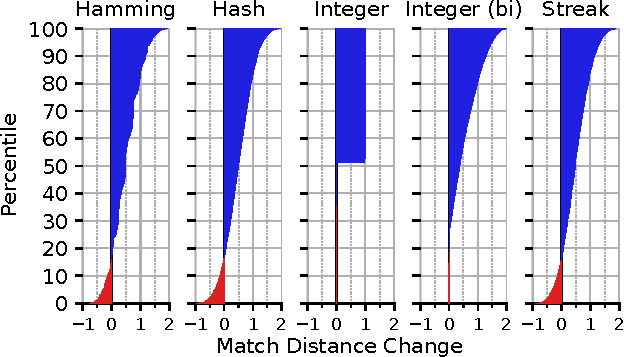
\includegraphics[width=\linewidth]{img/detour_difference/bitweight=0dot5+seed=1+title=low-triplet-analysis+_data_hathash_hash=6b0749ef97a58721+_script_fullcat_hash=2ded962cad675fe3+ext=}
\caption{
Cumulative distributions of sampled detour difference values.
Each distribution visualization arranges individually sampled observations (thin horizontal bars) vertically in descending order.
The $y$ axis can be interpreted as ranging from the \nth{0} percentile of outcomes (bottom) to \nth{100} percentile (top) with horizontal bar width showing the detour difference at a certain percentile.
A positive value (colored blue) indicates that total distance increased with the addition of an intermediate stop.
A value of exactly 0 indicates an intermediate stop had no effect on total distance.
A negative value (colored red) indicates violation of the triangle inequality: taking an intermediate stop reduced the total distance traveled.
}
\label{fig:detour_difference_supp}

\end{center}
\end{figure}


\begin{figure}
\begin{center}

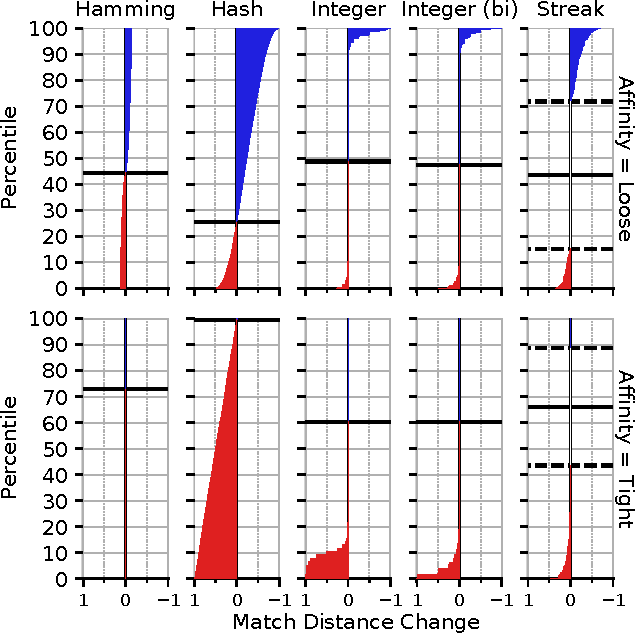
\includegraphics[width=\columnwidth]{img/mutational_step/bitweight=0dot5+seed=1+title=low-mutational-step+_data_hathash_hash=95a57768de56995a+_script_fullcat_hash=b9a24f3843e31e82+ext=}
\caption{
Distributions of mutation effects on match distance for loosely matched (pre-mutation match distance $> 0.5$) and tightly matched (pre-mutation match distance $< 0.01$) tag pairs.
Each distribution visualization arranges individually sampled observations of mutation outcome from an independently sampled tag pair (thin horizontal bars) vertically in descending order.
The $y$ axis can be interpreted as ranging from the \nth{0} percentile of outcomes (bottom) to \nth{100} percentile (top) with horizontal bar width showing the mutation effect size at a certain percentile.
Mutations that increase affinity are colored blue and mutations that decrease affinity are colored red.
Solid lines indicate the median between mutations that increase match distance and mutations that decrease match distance.
Dashed lines demarcate the boundaries between non-neutral and perfectly-neutral mutations.
Note that the $x$ axis is inverted so mutations increasing affinity fall to the right and mutations decreasing affinity fall to the left.
}
\label{fig:mutational_step_supp}

\end{center}
\end{figure}


\begin{figure}[]{\linewidth}
\centering
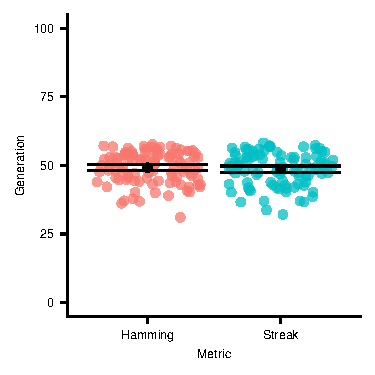
\includegraphics[width=\linewidth]{img/gp_results/panel-cst-times.pdf}%
\caption{
 CST TODO
 }
\label{fig:cst-times}
\end{figure}


\begin{figure*}
\begin{minipage}{6in}
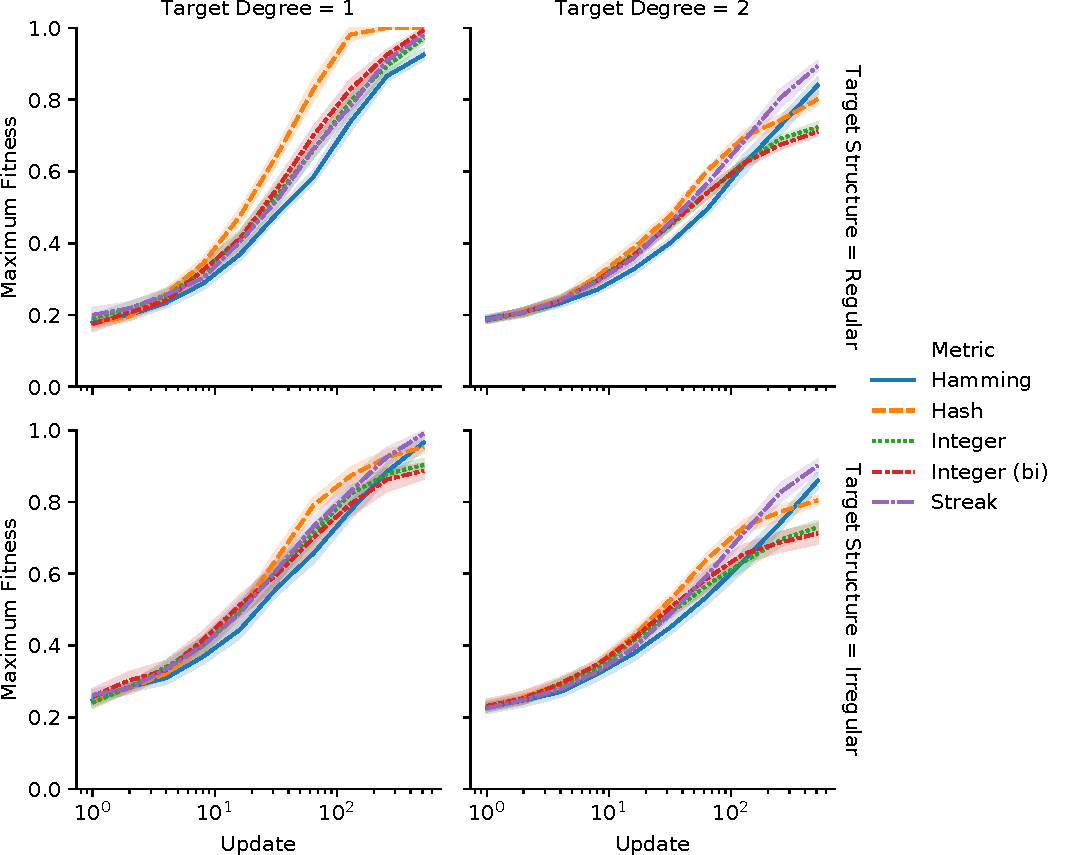
\includegraphics[width=\textwidth]{img/target_evolve_big/viz=max-fitness-line+_data_hathash_hash=4db1200f9d71a980+_script_fullcat_hash=fe3ddc711c5abfad+ext=}
\caption{64-node target graph}
\label{fig:evolve_big_bests}
\end{minipage}
\begin{minipage}{\textwidth}
\caption{
Trajectories of adaptive evolution for each tag-matching metric on the 64-node graph-matching task.
Maximum fitness represents the best fitness value for any individual within a population.
Here report using each metric's best-performing per-bit mutation rate.
(See Supplementary Figure \ref{fig:evolve_big_mutsweep} for survey showing how mutation rate affects adaptive evolution under each metric.)
Note log-scale x-axes.
Shaded area represents bootstrapped 95\% confidence intervals across 20 replicate observations.
}
\label{fig:evolve_bests64}
\end{minipage}
\end{figure*}


\begin{table}[!htbp]
\begin{tabular}{l|l|l|l}
\textbf{Metric}       & \textbf{Target Structure} & \textbf{Target Degree} &  \textbf{\begin{tabular}[c]{@{}l@{}}Best-Performing \\ Per-Genome Bit\\ Mutation Rate\end{tabular}} \\ \hline
Hash                  & Regular                   & 1                      & 0.75                                                                                         \\\hline
Hash                  & Regular                   & 2                      & 0.75                                                                                         \\\hline
Hash                  & Irregular                 & 1                      & 1.0                                                                                          \\\hline
Hash                  & Irregular                 & 2                      & 0.75                                                                                         \\\hline
Hamming               & Regular                   & 1                      & 4.0                                                                                          \\\hline
Hamming               & Regular                   & 2                      & 2.0                                                                                          \\\hline
Hamming               & Irregular                 & 1                      & 4.0                                                                                          \\\hline
Hamming               & Irregular                 & 2                      & 2.0                                                                                          \\\hline
Integer               & Regular                   & 1                      & 6.0                                                                                          \\\hline
Integer               & Regular                   & 2                      & 6.0                                                                                          \\\hline
Integer               & Irregular                 & 1                      & 8.0                                                                                          \\\hline
Integer               & Irregular                 & 2                      & 6.0                                                                                          \\\hline
Bidirectional Integer & Regular                   & 1                      & 4.0                                                                                          \\\hline
Bidirectional Integer & Regular                   & 2                      & 6.0                                                                                          \\\hline
Bidirectional Integer & Irregular                 & 1                      & 8.0                                                                                          \\\hline
Bidirectional Integer & Irregular                 & 2                      & 4.0                                                                                          \\\hline
Streak                & Regular                   & 1                      & 3.0                                                                                          \\\hline
Streak                & Regular                   & 2                      & 2.0                                                                                          \\\hline
Streak                & Irregular                 & 1                      & 3.0                                                                                          \\\hline
Streak                & Irregular                 & 2                      & 1.5                                                                             \end{tabular}

\caption{
Best-performing per-bit mutation rates for 64-vertex graph matching tasks.
See Supplementary Figure \ref{fig:evolve_big_mutsweep} for performance across surveyed mutation rates.
}
\label{tab:evo_graph_mut_big}


\end{table}


\begin{figure*}
\begin{center}

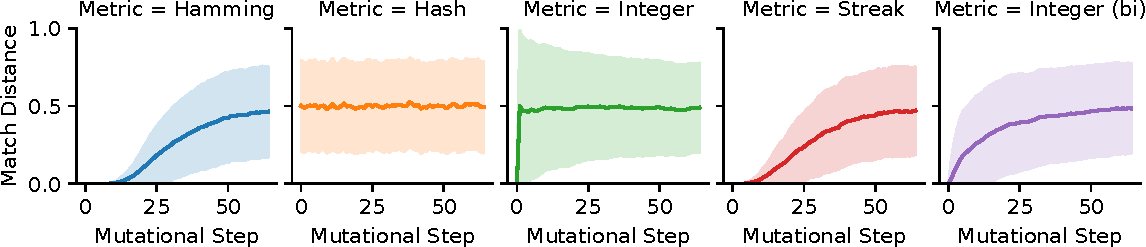
\includegraphics[width=\textwidth]{{{mutational_walk/bitweight=0.5+seed=1+title=mutational_walk_lineplot+_data_hathash_hash=ff15c8831d4f9288+_script_fullcat_hash=c872df869f05035a+ext=}}}
\caption{
TODO
}
\label{fig:mutational_walk_lineplot}

\end{center}
\end{figure*}


\begin{figure}[!htbp]
\begin{center}

\begin{subfigure}{\textwidth}
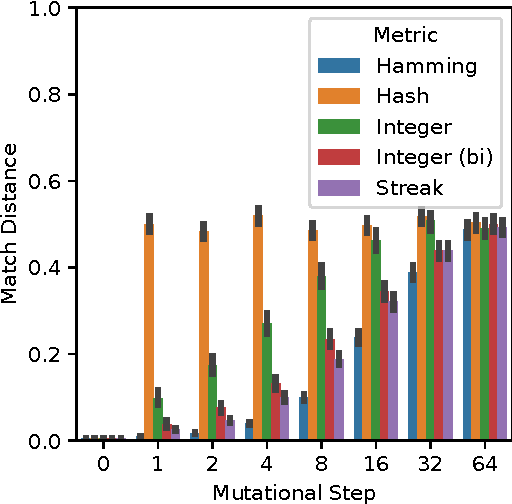
\includegraphics[width=\textwidth]{img/mutational_walk_sampled_start/bitweight=0dot5+seed=1+title=mutational_walk_barplot+_data_hathash_hash=05b961e08b5b7854+_script_fullcat_hash=982405ca713eba73+ext=}
\caption{
Error bars represent 95\% confidence intervals.
Note logarithmic scale on the $x$ axis.
}
\label{fig:mutational_walk_sampled_start_barplot}
\end{subfigure}

\begin{subfigure}{\textwidth}
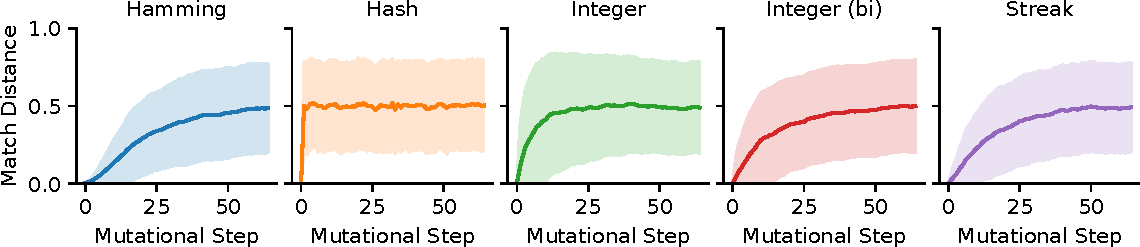
\includegraphics[width=\textwidth]{img/mutational_walk_sampled_start/bitweight=0dot5+seed=1+title=mutational_walk_lineplot+_data_hathash_hash=05b961e08b5b7854+_script_fullcat_hash=982405ca713eba73+ext=.pdf}
\caption{
Alternate visualization, shaded area represents standard deviation.
}
\end{subfigure}

\caption{
Match distance along mutational walks from 32-bit tags sampled for initial match distance $<0.01$.
}
\label{fig:mutational_walk_sampled_start}

\end{center}
\end{figure}


\begin{figure}
\begin{center}

\begin{subfigure}{\textwidth}
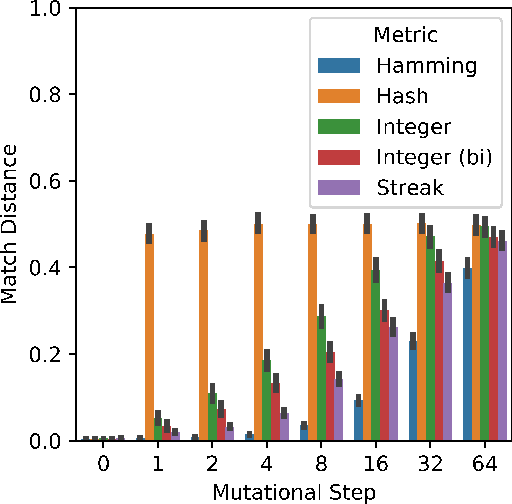
\includegraphics[width=\textwidth]{img/mutational_walk_sampled_start_64/bitweight=0dot5+seed=1+title=mutational_walk_barplot+_data_hathash_hash=2137b5ab8659c35e+_script_fullcat_hash=982405ca713eba73+ext=}
\caption{
Error bars represent 95\% confidence intervals.
Note logarithmic scale on the $x$ axis.
}
\label{fig:mutational_walk_sampled_start_64_barplot}
\end{subfigure}

\begin{subfigure}{\textwidth}
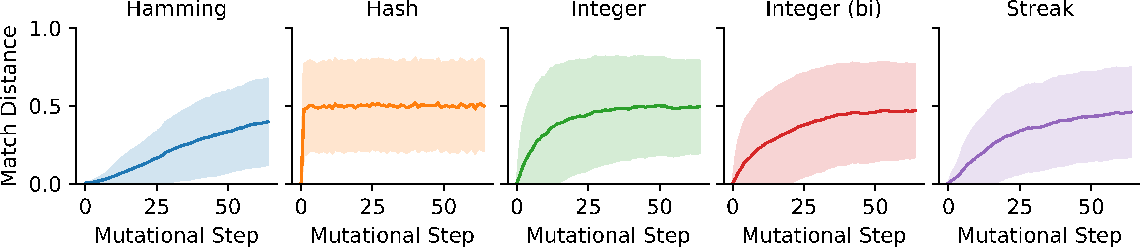
\includegraphics[width=\textwidth]{img/mutational_walk_sampled_start_64/bitweight=0dot5+seed=1+title=mutational_walk_lineplot+_data_hathash_hash=2137b5ab8659c35e+_script_fullcat_hash=982405ca713eba73+ext=}
\caption{
Alternate visualization, shaded area represents standard deviation.
}
\end{subfigure}

\caption{
Match distance along mutational walks from 64-bit tags sampled for initial match distance $<0.01$.
}
\label{fig:mutational_walk_sampled_start}

\end{center}
\end{figure}


\begin{figure*}[!htbp]
\begin{minipage}{6in}
\begin{center}

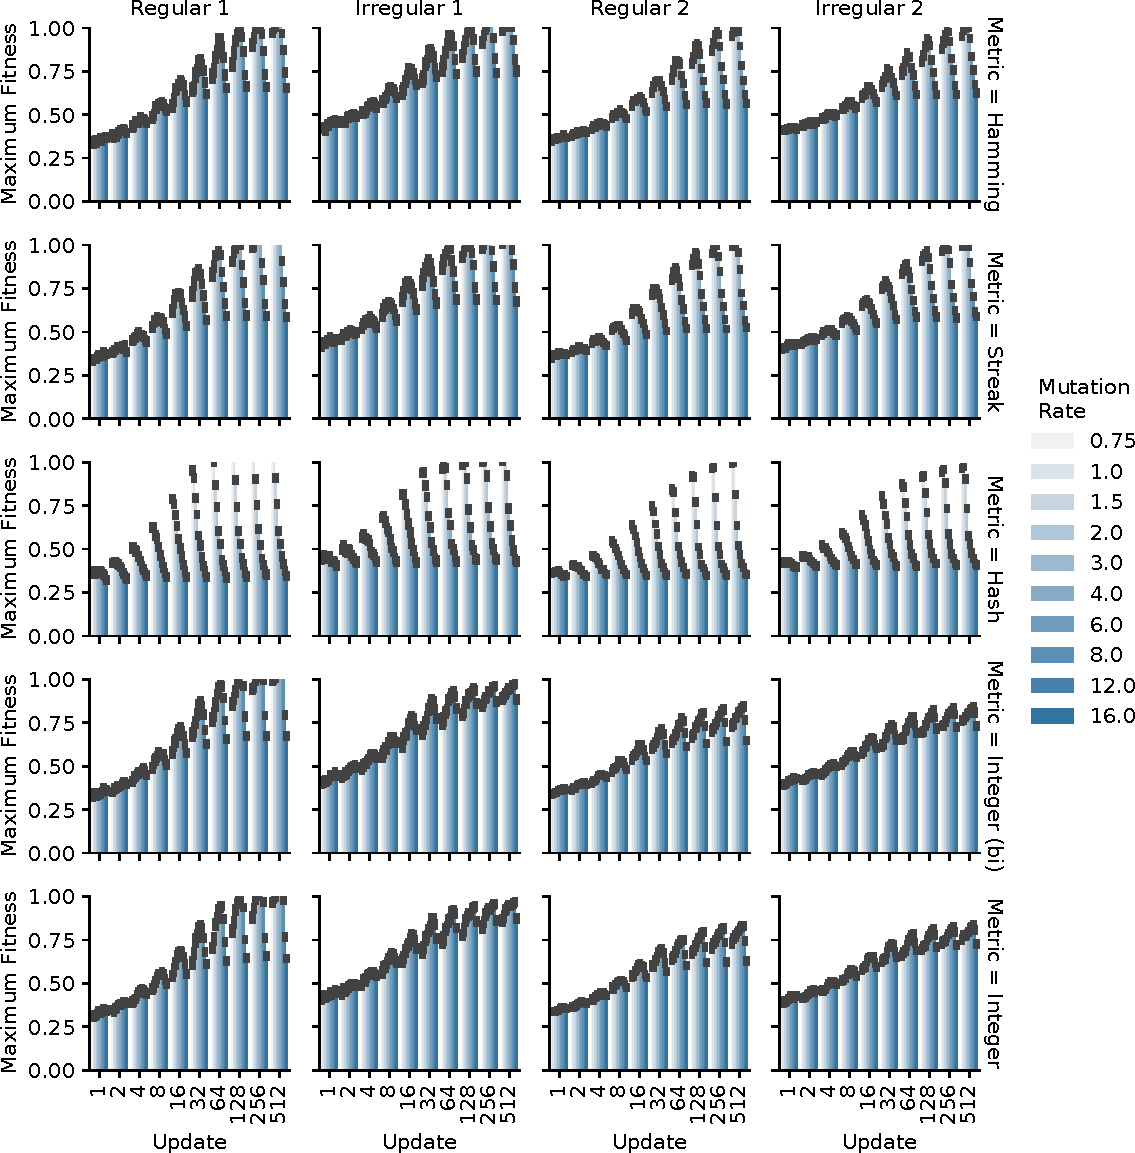
\includegraphics[width=\textwidth]{img/target_evolve/title=fitness_mutation_barplot+_data_hathash_hash=4c78832f20b46ffd+_script_fullcat_hash=6ccad43c80699be8+ext=}
\caption{
32-node graph-matching task mutation rate sensitivity analysis.
Metrics exhibited fastest adaptive evolution within the range of mutation rates surveyed, except the hash metric which exhibited fastest adaptive evolution at at the lowest mutation rate surveyed.
Maximum fitness is the best fitness value for any individual within a population.
Maximum fitness at each update is presented across the range of surveyed mutation rates.
Error bars represent bootstrap 95\% confidence intervals across 50 replicate populations.
}
\label{fig:evolve_mutsweep}

\end{center}
\end{minipage}
\end{figure*}


\begin{figure*}
\begin{center}

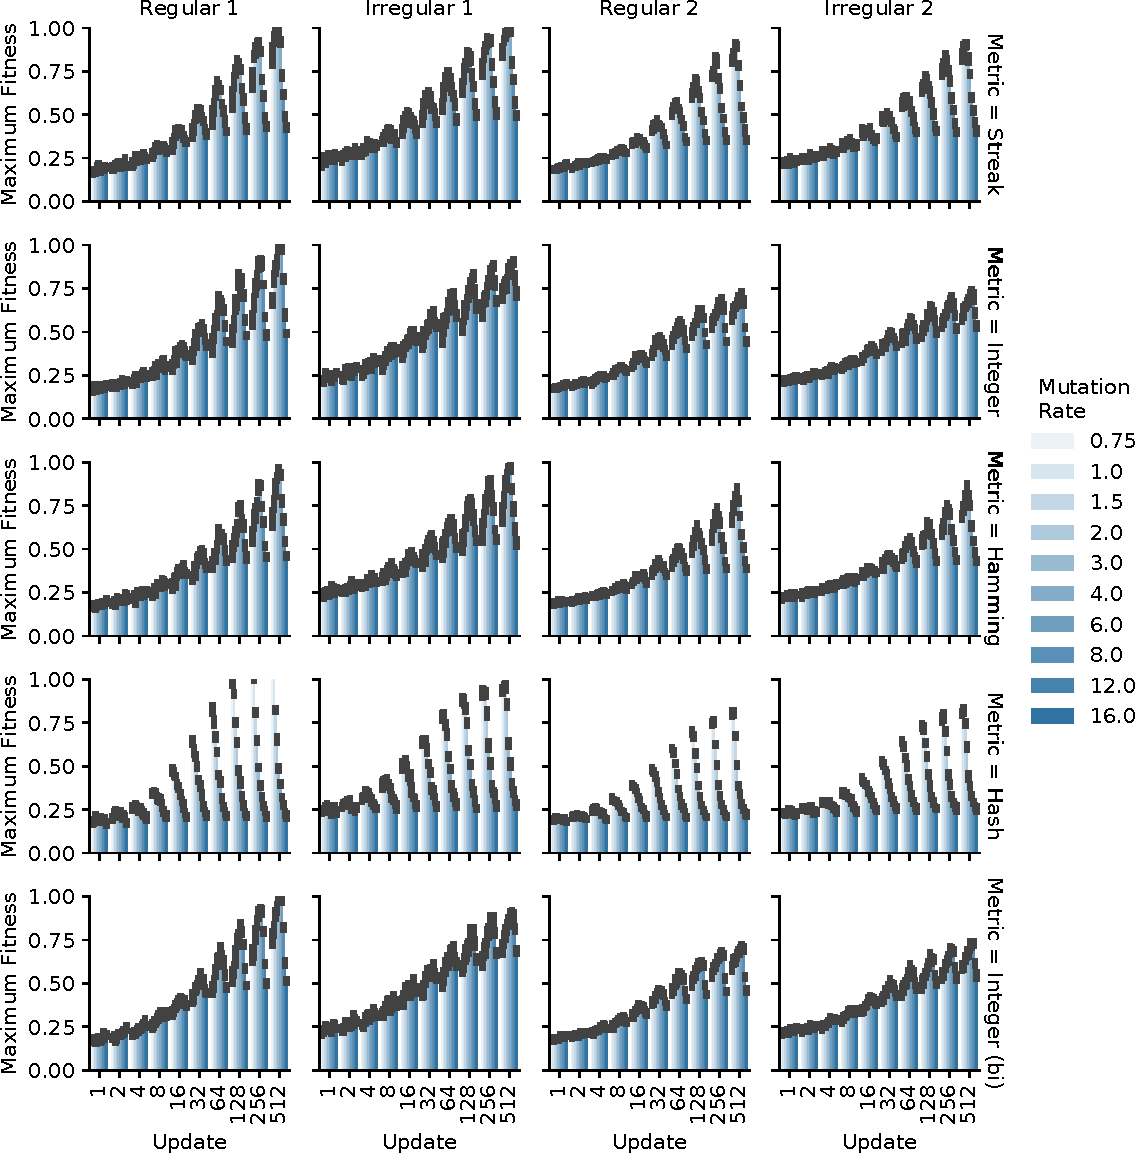
\includegraphics[width=\textwidth]{target_evolve_big/title=fitness_mutation_barplot+_data_hathash_hash=4db1200f9d71a980+_script_fullcat_hash=fe3ddc711c5abfad+ext=}
\caption{
Maximum fitness among replicate runs across a set of per-bit mutation rates.
Error bars represent 95\% confidence intervals.
}
\label{fig:evolve_mutsweep}

\end{center}
\end{figure*}


\pragmaonce

% adapted from https://www.overleaf.com/learn/latex/Commands
\newcommand{\dissertationelse}[2]{%
% adapted from https://tex.stackexchange.com/a/33577
\ifdefined\DISSERTATION
#1
\else
#2
\fi
}


\section{Genetic Programming Experiments}
\label{sec:gpsupplement}


\subsection{SignalGP}

SignalGP (Signal-driven Genetic Programs) is a GP representation that enables signal-driven (\textit{i.e.}, event-driven) program execution.
In SignalGP, programs are segmented into modules (functions) that may be automatically triggered by exogenously- or endogenously-generated signals.
Each module in SignalGP associates a tag with a linear sequence of instructions.
SignalGP makes explicit the concept of signals (events), which comprise a tag and, optionally, signal-specific data.
Signals trigger the module with the closest matching tag (according to a given tag-matching scheme), using any signal-associated data as input to the triggered module.
SignalGP can handle many signals simultaneously, processing each in parallel.

The SignalGP instruction set, in addition to including traditional GP operations, allows programs to generate internal signals, broadcast external signals, and otherwise work in a tag-based context.
Instructions contain arguments, including an evolvable tag, that may modify the instruction's effect, often specifying memory locations or fixed values.
Instructions may refer to program modules using tag-based referencing; for example, an instruction may trigger the execution of a program module using the instruction's tag to specify which module to trigger.
SignalGP also supports genetic regulation with promoter and repressor instructions that, when executed, allow programs to adjust how well subsequent signals match with a target function (specified with tag-based referencing).

See \citepinappendix{lalejini2018evolving} for a more detailed description of the SignalGP representation. Additionally, see the GitHub repository for the SignalGP implementation used in this work \citepinappendix{lalejini_2020_3781295}.

\subsection{Changing-signal Task Description}

The changing-signal task requires programs to express a distinct response to each of $K$ environmental signal (each signal has a unique tag).
Programs express a response by executing one of $K$ response instructions.
Successful programs can `hardcode' each response with the appropriate environmental signal, ensuring that each environmental signal's tag best matches the function containing the correct response.
We expect the particular metric used to match tags to influence how well programs adapt to changing-signal task.

During evaluation, we afford programs 64 time steps to express the appropriate response after receiving a signal.
Once a program expresses a response or the allotted time expires, we reset the program's virtual hardware (resetting all executing threads and thread-local memory), and the environment produces the next signal.
Evaluation continues until the program correctly responds to each of the $K$ environmental signals or until the program expresses an incorrect response.
During each evaluation, programs experience environmental signals in a random order; thus, the correct \textit{order} of responses will vary and cannot be hardcoded.

% Experiment overview
For each metric, we evolved 200 replicate populations (each with a unique random number seed) of 500 asexually reproducing programs in an eight-signal environment ($K=8$) for 100 generations.
We identified the most performant tag mutation rate (from a range of possible mutation rates) for each metric to use in our experiment.
These data (and analyses) are available online in the GitHub repository that houses these experiments \citepinappendix{lalejini_2020_3781295}.
We used the following per-bit tag mutation rates for the changing-signal task: 0.01 for the Hamming and Streak metrics, 0.002 for the Hash metric, and 0.02 for the Integer and Bidirectional Integer metrics.
Aside from tag mutation rate, the overall configuration used for each metric was identical.
We limited tag variation in offspring to tag mutation (bit flips) by initializing populations with a common ancestor program in which all tags are identical and by disallowing mutations that would insert instructions with random tags.

The full configuration details for the changing-signal task (including a guide to running these experiments on your local machine) can be found in the associated GitHub repository \citepinappendix{lalejini_2020_3781295}.

\subsection{Directional-signal Task Description}

% Task overview
As in the changing-signal task, the directional-signal task requires that programs respond to a sequence of environmental cues; in the directional-signal task, however, the correct response depends on previously experienced signals.
In the directional-signal task, there are two possible environmental signals --- a `forward-signal' and a `backward-signal' (each with a distinct tag) ---  and four possible responses.
If a program receives a forward-signal, it should express the next response, and if the program receives, a backward-signal, it should express the previous response.
For example, if response-three is currently required, then a subsequent forward-signal indicates that response-four is required next, while a backward-signal would instead indicate that response-two is required next.
Because the appropriate response to both the backward- and forward-signals change over time, successful programs must regulate which functions these signals trigger (rather than hardcode each response to a particular signal).

% Evaluation overview
We evaluate programs on all possible four-signal sequences of forward- and backward-signals (sixteen total).
For each program, we evaluate each sequence of signals independently, and a program's fitness is equal to its aggregate performance.
Otherwise, evaluation on a single sequence of signals mirrors that of the changing-signal task.

% Experiment overview
We used an identical experimental design for the directional-signal task as in the changing-signal task.
However, we evolved programs for 5000 generations (instead of 100) and re-parameterized each metric's tag mutation rate (these data are available in the associated GitHub repository \citepinappendix{lalejini_2020_3781295}):
0.001 for the Hamming and Hash metrics, 0.002 for the Integer and Streak metrics, and 0.0001 for the Bidirectional Integer Metric.

The full configuration details for the directional-signal task (including a guide to running these experiments on your local machine) can be found in the associated GitHub repository \dissertationelse{\citep{lalejini_2020_3781295}}{\citepinappendix{lalejini_2020_3781295}}.

\subsection{Data analysis and Implementation}

The source code for our GP experiments can be found in the following GitHub repository: \dissertationelse{\citep{lalejini_2020_3781295}}{\citepinappendix{lalejini_2020_3781295}}. This repository additionally includes all data analysis and visualization scripts, experiment configuration details, and a guide for running our experiments locally.



\footnotesize
\bibliographystyleinappendix{apalike}
\bibliographyinappendix{bibl} % replace by the name of your .bib file

\end{document}
